\subsection{Processo di infrastruttura}
\label{subsec:proc_infrastruttura}
Il processo di infrastruttura ha il compito di definire e mantenere l'infrastruttura e gli strumenti necessari allo svolgimento di tutti gli altri processi di ciclo di vita.

\subsubsection{Documentazione}
L'infrastruttura del processo di documentazione contiene tutti gli strumenti software, i linguaggi e i pacchetti usati per la stesura, la compilazione e la distribuzione dei documenti.

\paragraph{Linguaggio}
\label{par:latex}
Per stesura dei documenti è stato deciso di utilizzare LaTeX.
LaTeX è un linguaggio di markup per la creazione di testi basato sul software di composizione tipografica chiamato TeX.
LaTeX è il linguaggio più utilizzato per la produzione di documenti in formato PDF professionali.


\paragraph{Distribuzione TeX}
Il gruppo sviluppando la documentazione su sistema operativo Windows ha scelto l'utilizzo della distribuzione TeX chiamata \textbf{TeX Live}.
Questa distribuzione oltre che contenere TeX fornisce pacchetti, font e software a supporto tra cui un gestore di pacchetti grafico chiamato \textbf{TLShell}.
L'installazione di TeX Live può essere fatta seguendo le istruzioni indicate al link \href{https://www.tug.org/texlive/windows.html}{Installazione Tex Live}.

\subparagraph{TLShell}
\label{subpar:TLShell}
L'installazione di pacchetti tramite TLShell è abbastanza intuitiva e segue i passaggi:
\begin{enumerate}
    \item Avvio TLShell.
    \item Selezionare il radio button \texttt{Not installed} \hyperref[fig:installazione_pacchetti]{Figura \ref{fig:installazione_pacchetti} (1)}.
    \item Indicare il nome del pacchetto da installare nella barra di ricerca \hyperref[fig:installazione_pacchetti]{Figura \ref{fig:installazione_pacchetti} (2)}.
    \item Selezionare il radio button del pacchetto da installare \hyperref[fig:installazione_pacchetti]{Figura \ref{fig:installazione_pacchetti} (3)}.
    \item Cliccare il pulsante \texttt{Install marked} \hyperref[fig:installazione_pacchetti]{Figura \ref{fig:installazione_pacchetti} (4)}.
\end{enumerate}
\begin{figure}[H]
    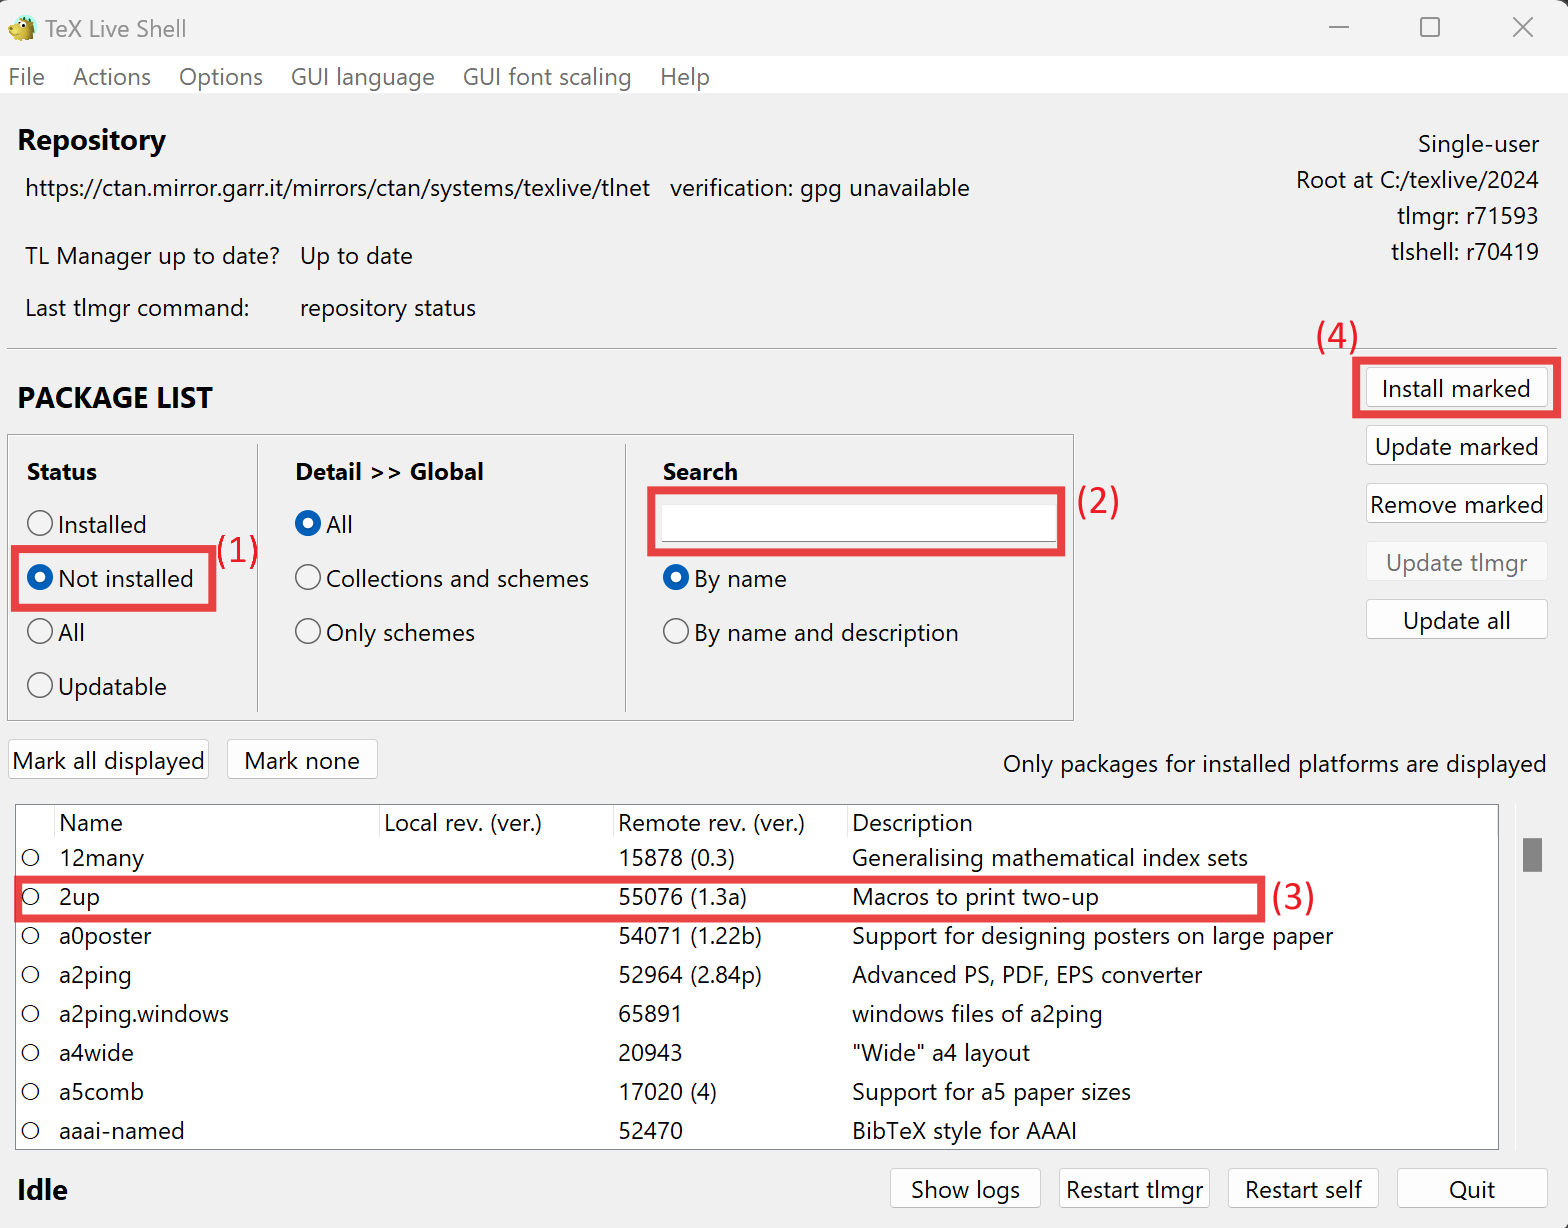
\includegraphics[scale=0.7]{Sezioni/ProcessiDiSupporto/Immagini/installazione_pacchetti.png}
    \caption{Installazione pacchetti LaTeX..}
    \label{fig:installazione_pacchetti}
\end{figure}

\paragraph{Comandi di base}
\label{par:comandi_di_base}
Di seguito vengono elencati i comandi di base che devono essere noti per la stesura di documenti in LaTeX.

\subparagraph{Tabelle}
\label{subpar:tabelle}
\begin{lstlisting}

        \begin{table}[H]
            \begin{tabularx}[| X | c | l | r |]
                \hline
                \makecell{Intestazione1 \\ Intestazione1} &
                Intestazione2 &
                Intestazione3 &
                Intestazione4 \\

                \hline

                prima colonna prima riga   &
                seconda colonna prima riga &
                terza colonna prima riga  &
                quarta colonna prima riga  &

                \hline

                ...

                \hline
            \end{tabularx}
            \caption{Riassunto contenuto.}
        \end{table}
\end{lstlisting}
Dove:
\begin{itemize}
    \item \lstinline+[H]+ indica che il posizionamento della tabella nel pdf deve essere dove si trova nel codice.
    
    \item \lstinline+[| X | c | l | r |]+ indica le colonne della tabella.

    \lstinline+|+ indica una riga di separazione tra le colonne.

    \lstinline+X+ indica una colonna che si allarga dinamicamente.

    \lstinline+c+, \lstinline+l+ e \lstinline+r+ indicano rispettivamente colonne in cui il posizionamento del testo è centrale, a sinistra e a destra.
    
    \item \lstinline+\makecell{... \\ ...}+ permette di creare celle con testo su più righe, usando \textbackslash\textbackslash{} per andare a capo. 

    \item \lstinline+\hline+ crea una linea orizzontale.
\end{itemize}

\subparagraph{Link}
Link a elementi interni alla pagina:
\begin{lstlisting}
    \label[sec:nome]

    ... 

    \hypperref[sec:nome]{nomeLink}
\end{lstlisting}
Dove:
\begin{itemize}
    \item Convezione standard per nominare le label: \texttt{tipoElemento:nome}.
    Dove i possibili tipi di elemento sono: paragraph(par), subparagraph(subpar), section(sec), subsection(subsec) e figure(fig).
\end{itemize}
\noindent Link a elementi esterni alla pagina:
\begin{lstlisting}
    \href{URL}{nomeLink}
\end{lstlisting}

\subparagraph{Listati di codice}
Listati di codice su più righe:
\begin{lstlisting}[mathescape=true]
\begin{lstlisting}
    ...
\$$end{lstlisting}
\end{lstlisting}
\noindent 
Listati di codice inline:
\begin{lstlisting}
    \texttt{code}
    \lstinline+code+
\end{lstlisting}

\subparagraph{Figure}
\begin{lstlisting}
    \begin{figure}[H]
        \includegraphics[scale=1.2]{pathImmagine}
        \caption{Riassunto immagine.}
        \label{fig:IdFigura}
    \end{figure}
\end{lstlisting}
Dove:
\begin{itemize}
    \item \texttt{[H]} permette di posizionare la figura nel pdf dove si trova nel codice.
    \item \texttt{scale=x.y} indica la scala da applicare all'immagine.
\end{itemize}

\subparagraph{Inclusione file}
L'inclusione di file .tex permette di dividere un documento in più file rendendone la modifica più semplice.
\begin{lstlisting}
    \input{PercorsoAlFile}
\end{lstlisting} 

\subparagraph{Grafici}
\label{subpar:grafici}
\begin{lstlisting}


\begin{axis}[
    title={Titolo del grafico},
    xlabel={Nome dell'asse x}, 
    ylabel={Nome dell'asse y},
    xmin=, xmax=,  
    ymin=, ymax=,
    xtick={assex1, assex2, ...},
    ytick={assey1, assey2, ...},
    grid=, 
    grid style={},
    width=, height=, 
    legend pos= 
]

\addplot[color=] coordinates {
    (x1, y1) (x2, y2) ...
};
\addlegendentry{}

\end{lstlisting}

Dove:
\begin{itemize}
    \item \lstinline+title+ indica il titolo del grafico. 
    
    \item \lstinline+xlabel+ e \lstinline+ylabel+ indicano i nomi degli assi x e y. 
    
    \item \lstinline+xmin+ e \lstinline+xmax+ indicano i valori minimi e massimi dell'asse x. 

    \item \lstinline+ymin+ e \lstinline+ymax+ indicano i valori minimi e massimi dell'asse y.
    
    \item \lstinline+xtick+ e \lstinline+ytick+ indicano i valori sull'asse x e y.
    
    \item \lstinline+grid+ indica se mostrare la griglia che può essere \texttt{major}, \texttt{minor} o \texttt{both}.
    
    \item \lstinline+grid style+ indica lo stile della griglia che può essere \texttt{dotted}, \texttt{dashed}, \texttt{solid}, \texttt{none} e se ne può specificare il colore, es. \texttt{gray}.
     
    \item \lstinline+width+ e \lstinline+height+ indicano la larghezza e l'altezza del grafico.
     
    \item \lstinline+legend pos+ indica la posizione della legenda che può essere \texttt{north east}, \texttt{north west}, \texttt{south east}, \texttt{south west}.
    
    \item \lstinline+addplot+ \lstinline+coordinates+ indica i valori da aggiungere al grafico.
    
    \item \lstinline+[]+ subito dopo addplot contiene le caratteristiche del grafico tracciato, come il colore.
    
    \item \lstinline+addlegendentry+ indica il nome del grafico tracciato.
\end{itemize}



\paragraph{Pacchetto LaTeX}
Per rendere i file sorgenti meno complessi è stato deciso di definire un pacchetto LaTeX che contiene:
\begin{enumerate}
    \item La definizione di comandi e ambienti di uso comune.
    \item Le dichiarazioni dei pacchetti usati.
\end{enumerate}
Oltre a diminuire la verbosità dei documenti questo metodo permette di centralizzare la gestione dei pacchetti, dei comandi e degli ambienti semplificando la manutenzione.
I pacchetti usati devono essere installati manualmente usando il processo spiegato nella sezione \hyperref[subpar:TLShell]{TLShell}.
In \hyperref[fig:pacchetto_latex]{Figura \ref{fig:pacchetto_latex}} viene mostrata la struttura del pacchetto LaTeX.
\textbf{Nota bene}: Il pacchetto per poter essere importato deve essere indicato con il comando \lstinline|\usepackage| e il suo percorso deve essere indicato nella variabile di ambiente TEXINPUTS.
La spiegazione della configurazione dell'ambiente per l'utilizzo del pacchetto è spiegata nella sezione \hyperref[par:IDE]{Integrated Development Environment IDE}.
\begin{figure}[H]
    \dirtree{%
        .1 Packages.
        .2 Immagini.
        .3 logo.jpeg.
        .2 custom.sty.
        .2 TitlePage.tex .
    }
    \caption{Struttura pacchetto LaTeX.}
    \label{fig:pacchetto_latex}
\end{figure}

\subparagraph{Comandi personalizzati}
\label{subpar:comandi_personalizzati}
Nel pacchetto sono definiti i seguenti comandi necessari per la scrittura di un documento:
\begin{enumerate}
    \item \lstinline|\primapagina|\ : inserisce nella posizione di invocazione la pagina iniziale dei documenti.
    Questo comando sfrutta le variabili indicate alla sezione \hyperref[par:struttura_di_base_documenti]{Struttura di base documenti}.
    \item \lstinline|\glossario{<termine>}|\ : modifica lo stile del termine per indicare la sua presenza nel glossario    
\end{enumerate}
Per la stesura delle descrizioni dei casi d'uso il gruppo ha deciso di definire un insieme di comandi da utilizzare all'interno del ambiente personalizzato \lstinline|\begin{usecase} ...\end{usecase}|:
\label{subpar:casi_uso}
\begin{enumerate}
    \item \lstinline|\req{<link requisito utente>}|: genera in automatico la riga della tabella relativa al requisito di riferimento.
    \item \lstinline|\pre{ \item <pre condizione 1> ... }|: genera in automatico la riga delle pre-condizioni mostrandole in una lista.
    \item \lstinline|\post{ \item <post condizione 1> ... }|: genera in automatico la riga delle post-condizioni mostrandole in una lista.
    \item \lstinline|\actor{<attore principale>}|: genera in automatico la riga per l'attore principale.
    \item \lstinline|\subactors{<attori secondari>}|: genera in automatico la riga per gli attori secondari.
    \item \lstinline|\trigger{<trigger>}|: genera in automatico la riga per il trigger.
    \item \lstinline|\inc{<casi d'uso inclusi>}|: genera in automatico la riga per i casi d'uso inclusi.
    \item \lstinline|\base{<caso d'uso base>}|: genera in automatico la riga per il caso d'uso base.
    \item \lstinline|\scenario{\item <azione 1> ...}|: genera in automatico la riga per lo scenario principale e la popola indicando le azioni in una lista.
    \item \lstinline|\subscenario{\item <condizione 1> ...}|: genera in automatico la riga per per gli scenari secondari e la popola indicandoli in una lista.
\end{enumerate}

\subparagraph{Ambienti personalizzati}
\label{subpar:ambienti_personalizzati}
Il pacchetto definisce anche i seguenti ambienti necessari per la scrittura di un documento:
\begin{enumerate}
    \item \lstinline|\begin{registromodifiche} ... \end{registromodifiche}|\ :
    permette di definire il registro delle modifiche tralasciando le impostazioni della tabella.
    All'interno di questo ambiente devono essere indicate le righe del \hyperref[par:registro_delle_modifiche]{registro delle modifiche}.
    \item \lstinline|\begin{usecase}{<id>}{<descrizione>} ... \end{usecase}|:
    genera in automatico la tabella per la descrizione dei casi d'uso.    
\end{enumerate}

\paragraph{Struttura di base documenti}
\label{par:struttura_di_base_documenti}
Di seguito viene mostrato il codice necessario per la definizione dello scheletro di un documento soggetto al processo di \hyperref[subsec:gestione_della_configurazione]{Gestione della configurazione}:

\begin{lstlisting}
\documentclass[a4paper, 12pt]{article}
\usepackage{custom}

%--------------------VARIABILI--------------------
\def\lastversion{ Versione documento }
\def\title{ Nome documento }
\def\date{ Data }
%------------------------------------------------

\begin{document}

\primapagina

\begin{registromodifiche}

\end{registromodifiche}

\tableofcontents

\newpage
\end{document}
\end{lstlisting}
\textbf{Nota bene}: I valori delle variabili devono seguire le regole indicate nelle sezioni \hyperref[subsec:documentazione]{Documentazione} e \hyperref[par:versione_documenti]{Versione dei documenti}.

\subparagraph{Gestione documenti "lunghi"}
Per rendere più semplice la gestione di documenti molto lunghi il gruppo ha deciso di dividerene il contenuto in più file .tex.
I documenti soggetti a questa divisione sono:
\begin{enumerate}
    \item Norme di progetto.
    \item Analisi dei requisiti.
    \item Piano di progetto.
\end{enumerate}
Ognuno di questi file verrà diviso in sezioni contenute in una cartella avente nome uguale al documento in Pascal case.
Queste cartelle sono contenute nella cartella padre comune \texttt{Sezioni}.
Le sezioni saranno divise a loro volta in sottosezioni contenute nella cartella \texttt{Sottosezioni}.
Inoltre ogni cartella di sottosezione conterrà una cartella chiamata \texttt{Immagini}.
La divisione segue la struttura indicata in \hyperref[fig:struttura_file_lungi]{Figura \ref{fig:struttura_file_lungi}} dove \texttt{F} indica il nome di un file da dividere:

\begin{figure}[H]
    \dirtree{%
    .1 cartella di F.
    .2 F.tex.
    .2 Sezioni.
    .3 SezioneA.
    .4 SezioneA.tex.
    .4 Sottosezioni.
    .5 Sottosezione\_a.tex.
    .5 Sottosezione\_b.tex.
    .4 Immagini.
    .3 SezioneB.
    .4 SezioneB.tex.
    .4 Sottosezioni.
    .5 Sottosezione\_a.tex.
    .5 Sottosezione\_b.tex.
    .4 Immagini.
    }
    \caption{Struttura file "lunghi".}
    \label{fig:struttura_file_lungi}
\end{figure}


\paragraph{Integrated Development Environment IDE}
\label{par:IDE}
Come IDE per la stesura della documentazione viene utilizzato Visual Studio Code che può essere installato seguendo le istruzioni al seguente link \href{https://code.visualstudio.com/docs/setup/windows}{VsCode}.

Visual Studio Code dispone di un grande numero di estensioni che lo rendono molto versatile.
In particolare sono stati scelti dal gruppo le seguenti estensioni:
\begin{enumerate}
    \item \textbf{LaTeX Workshop}: \href{https://github.com/James-Yu/latex-workshop/wiki}{https://github.com/James-Yu/latex-workshop/wiki}.
    \item \textbf{LTeX+}: \href{ https://ltex-plus.github.io/ltex-plus}{ https://ltex-plus.github.io/ltex-plus}.
\end{enumerate}

\subparagraph{LaTeX Workshop}
Questa estensione permette di integrare la compilazione dei file LaTeX in Visual Studio Code.
LaTeX Workshop richiede che sia installato TeX Live.
Dopo aver installato l'estensione è necessario modificare la procedura di compilazione di modo che vengano cercati i pacchetti usati e i file .tex importati nella cartella Packages.
Per fare ciò è necessario seguire le azioni:
\begin{enumerate}
    \item Aprire Visual Studio Code.
    
    \item Premere la combinazioni di tasti \texttt{Ctrl+,}.
    
    \item Scrivere sulla barra di ricerca il testo \texttt{latex-workshop.tools} \hyperref[fig:texinputs]{Figura \ref{fig:texinputs} (1)}.
    
    \item Cliccare il link \texttt{Edit in settings.json} del primo risultato \hyperref[fig:texinputs]{Figura \ref{fig:texinputs} (2)}.
    
    \item Aggiungere al oggetto tool chiamato \texttt{latexmk} a seguito dell'attributo \texttt{args} l'attributo \texttt{env} indicando il seguente attributo \hyperref[fig:texinputs]{Figura \ref{fig:texinputs} (3)}: 
    \begin{lstlisting}
        "TEXINPUTS":"%WORKSPACE_FOLDER%/Packages;"
    \end{lstlisting}
\end{enumerate}

\begin{figure}[H]
    \center
    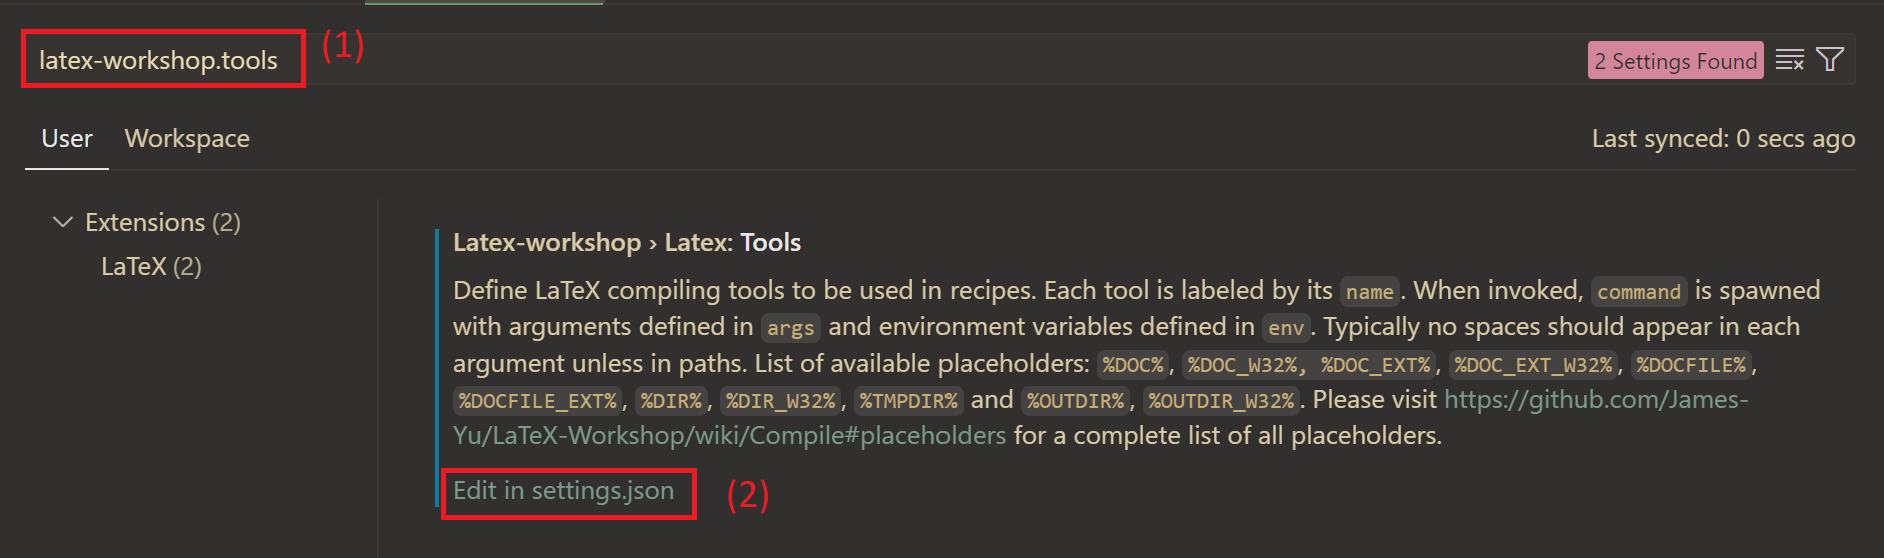
\includegraphics[scale=0.4]{Sezioni/ProcessiDiSupporto/Immagini/texinputs_setup.png}
    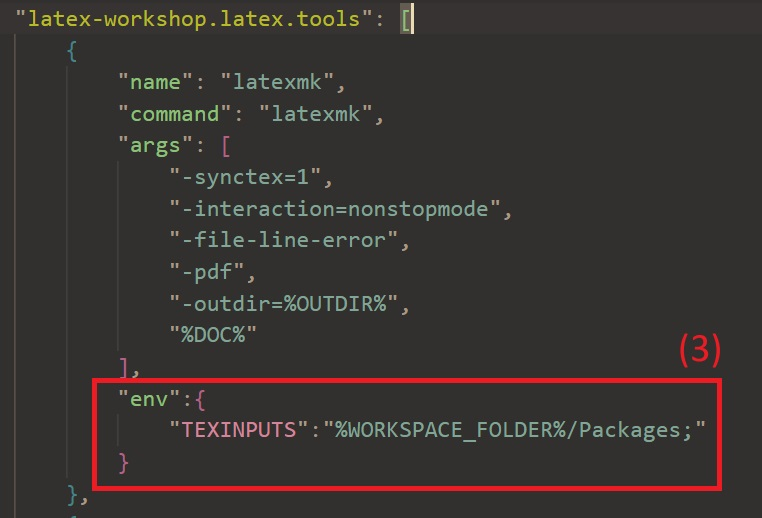
\includegraphics[]{Sezioni/ProcessiDiSupporto/Immagini/texinputs_setup_json.jpg}
    \caption{Modifica impostazioni LaTex Workshop.}
    \label{fig:texinputs}
\end{figure}
\textbf{Nota bene}: Per riuscire ad accedere al pacchetto locale è necessario lavorare in Visual Studio Code usando come "workspace folder" la cartella relativa alla repository.

\subparagraph{LTeX+}
LTeX+ è un'estensione che esegue lo "spell checking" dei documenti .tex per installarla basta cercarla nel marketplace di Visual Studio Code.
Per eventuali problemi di set up le procedure sono spiegate in modo chiaro e dettagliato al link \href{https://ltex-plus.github.io/ltex-plus/vscode-ltex-plus/setting-scopes-files.html}{installazione LTeX+}.

\subsubsection{Gestione della configurazione}
A supporto del processo di gestione della configurazione il gruppo ha scelto l'utilizzo di due strumenti:
\begin{enumerate}
    \item Git: \href{https://git-scm.com/doc}{https://git-scm.com/doc}.
    \item GitHub: \href{https://docs.github.com/en}{https://docs.github.com/en}.
\end{enumerate}

\paragraph{Git}
Git è un Distributed Version Control System DVCS  utilizzabile tramite interfaccia a linea di comando.
I DVCS hanno la caratteristica di permettere ai membri del gruppo di lavoro di mantenere una propria copia locale del repository e della sua storia.
Una volta modificata la copia locale del repository è necessario registrare le modifche nella copia centralizzata del repository.
Le operazioni e gli elementi di base comuni a tutti i DVCS: \textbf{repository}, \textbf{ramo}, \textbf{push}, \textbf{pull}, \textbf{conflitto} e \textbf{commit}.
Nelle sezioni succesive viene mostrato come Git implementa questi concetti e altri concetti caratteristici.

\subparagraph{repository}
Un repository in Git è una cartella contenente:
\begin{enumerate}
    \item Una cartella \texttt{.git} che contiene l'insieme di strutture dati e file necessari per la gestione della storia delle versioni dei file utente.
    \item Un insieme di file utente e cartelle di cui Git deve tenere la storia delle versioni.
\end{enumerate}
In git esistono due diverse declinazioni di repository:
\begin{enumerate}
    \item \textbf{remota}: esiste in un server remoto a cui i membri del team possono attingere tramite le operazioni di push e pull.
    
    \item \textbf{locale}: esiste solo sul file system locale e può essere associata ad un repository remoto usato come default per le operazioni di psuh e pull. 
\end{enumerate} 
Per creare un repository è possibile eseguire uno dei seguenti comandi:
\begin{lstlisting}
    git clone <URL>
    git init <NomeRepository>
\end{lstlisting}
Dove:
\begin{enumerate}
    \item Il primo comando permette di copiare la repository remota nella current working directory proprio file system.
    \item Il secondo comando permette di creare una repository nella current working directory nel proprio file system.
\end{enumerate}

\subparagraph{commit}
\label{subpar:commit}
Un commit rappresenta una istantanea del contenuto di uno o più file utente di cui è stata indicata l'esistenza a Git.
In Git ogni commit è associato alle seguenti informazioni:
\begin{enumerate}
    \item \textbf{hash SHA-1}: sequenza di 40 caretteri alfanumerici che identifica univocamente il commit all'interno del repository.
    \item \textbf{autore}.
    \item \textbf{data di creazione}.
    \item \textbf{messaggio}: usato per segnalare cosa fa il contenuto del commit.
    \item \textbf{commit padre}: hash SHA-1 dei commit padre.
\end{enumerate}
I commit sono quindi messi in relazione "padre-figlio" da Git andando a creare un albero.
L'unico commit che non ha padre è il primo commit chiamato \textbf{commit radice}.
I commit con più di un padre sono dei commit generati da operazioni di \hyperref[subpar:merge]{merge}.
Il comando Git per generare un commit con commento è:
\begin{lstlisting}
    git commit -m "<commento>"
\end{lstlisting}
Per comprendere meglio i commit leggere sezione \hyperref[subpar:3_aree_git]{3 aree di Git}.
Questo comando utilizza come commit padre il commit foglia del ramo corrente. 

\subparagraph{ramo}
\label{subpar:branch}
Un ramo in Git è un commit a cui è stata associata un etichetta mobile che funziona da alias per lo stesso.
Tramite questa etichetta mobile è possibile fare riferimento al commit ad essa associato.
Un ramo è un etichetta mobile nel senso che Git la sposta in automatico quando viene generato un commit figlio.
Questo crea una biforcazione nella storia dei commit(ramo) dove l'etichetta punta sempre all'ultimo commit(foglia) del nuovo flusso.

Git mantiene internamente un puntatore all'etichetta del ramo corrente chiamato commit \textbf{HEAD}.
Così facendo riesce ad operare nel modo atteso quando si eseguono comandi che agiscono rispetto al ramo corrente.
Git permette di ottenere riferimenti a commit padre del commit HEAD tramite le seguenti sintassi:
\begin{lstlisting}
    # riferimento al commit padre di HEAD
    # si possono concatenare arbitrari ^
    HEAD^

    # riferimento ad n-esimo parente di HEAD
    HEAD~n
\end{lstlisting}
 

Per creare un ramo esiste il comando:
\begin{lstlisting}
    git branch <nomeRamo>
\end{lstlisting}
Per eliminare un ramo esiste il comando:
\begin{lstlisting}
    # il ramo non deve avere commit
    git branch -d <nomeRamo>

    # il ramo puo avere commit
    git branch -D <nomeRamo>
\end{lstlisting}
Per spostarsi in un ramo esiste il comando:
\begin{lstlisting}
    git checkout <nomeRamo>
\end{lstlisting}
Per ottenere una lista dei rami del repository locale esiste il comando:
\begin{lstlisting}
    git branch
\end{lstlisting}
Per ottenere una lista dei rami dei repository locale e remoto è necessario applicare l'opzione \texttt{-a} al comando precedente.


\subparagraph{3 aree di Git}
\label{subpar:3_aree_git}
Git lavora su tre diversi livelli:
\begin{enumerate}
    \item \textbf{Commit HEAD}: rappresenta il ramo corrente.
    Per gestire il ramo corrente esistono i seguenti comandi:
    \begin{lstlisting}
    # modifica etichetta ramo correte usando il
    # commit indicato le modifiche vengono 
    # eliminate dal file system
    git reset --hard <hashCommit>

    # modifica etichetta ramo correte usando il
    # commit indicato le modifiche tornano 
    # nell'area di staging 
    git reset --soft <hashCommit>

    # ottenere la storia dei commit 
    # del ramo corrente
    git log --graph
    
    # ottenere la storia dei commit 
    # di tutti i rami
    git log --all --graph

    # ottenere differenze con area di staging
    git diff --cached
    
    # ottenere differenze con albero di lavoro
    git diff HEAD
    \end{lstlisting}
    
    \item \textbf{Area di staging}: anche chiamata indice o cache, è una struttura dati dinamica che contiene le modifiche ai file utente che Git deve aggiungere nel prossimo commit.
    
    Di seguito vengono mostrati i comandi per la gestione dell'area di staging:
    \begin{lstlisting}
    # aggiunge file
    git add <percorsoFile>

    # rimuove i file separati da ,
    git checkout -- <files>

    # ottenere differenze con albero di lavoro
    git diff 
    \end{lstlisting}
    
    \item \textbf{Albero di lavoro}: albero di cartelle e file che Git "conosce" e quindi ritiene come facenti parte del repository.
    
    Questi file e cartelle vengono chiamati \textbf{file tracciati} e devono per forza essere memorizzati all'interno della cartella relativa al repository.

    Un file diventa tracciato quando è passato dall'area di staging.
\end{enumerate}


\subparagraph{push}
\label{subpar:push}
L'operazione di push permette di pubblicare le modifiche apportate ad un repository locale al repository remoto a cui è associato.
Le declinazioni del comando di Git che permette di eseguire un push sono:
\begin{lstlisting}
    # pubblica il contenuto del ramo locale 
    # corrente nel ramo remoto indicato
    git push origin <ramoDestinazione> 

    # pubblica il contenuto del ramo locale
    # indicato nel ramo remoto indicato
    git push <ramoSorgente> origin <ramoDestinazione>
\end{lstlisting}   
Dove \texttt{origin} è il nome di default del riferimento al repository remoto e può essere gestiti usando i comandi:
\begin{lstlisting}
    # aggiunge nuovo riferimento remoto
    git remote add <nome> <URL>

    # rimuove il riferimento remoto
    git remote remove <nome>

    # modifica il riferimento remoto
    git remote set-url <nome> <URL>
\end{lstlisting}

\subparagraph{pull}
\label{subpar:pull}
L'operazione di pull permette aggiornare un repository locale con le modifiche registrate al repository remoto a cui è associato.
Git per eseguire un operazione di pull mette a dispozione il seguente comando:
\begin{lstlisting}
    # esegue il pull del ramo remoto indicato
    # nel ramo locale corrente
    git pull origin <nomeRamo>
\end{lstlisting}
In realà il comando \lstinline|git pull| è un comando composto che accorpa i comandi:
\begin{enumerate}
    \item \lstinline|git fetch origin <nomeRamo>|: recupera localmente il ramo remoto indicato.
    \item \lstinline|git merge <nomeRamo>|.
\end{enumerate}

\subparagraph{merge}
\label{subpar:merge}
L'operazione di merge esegue una fusione di due o più rami sorgente verso un ramo di destinazione.
A seguito dell'operazione di merge la cronologia del ramo di destinazione conterrà le modifiche dei rami sorgente.
In una fusione possono accadere le seguenti situazioni:
\begin{enumerate}
    \item I commit HEAD dei rami contengono file con nomi uguali ma contenuto diverso.
    In questo caso sorge un \textbf{conflitto}.

    \item Non esistono conflitti.

    \item Il commit HEAD del ramo di destinazione è in dietro rispetto ai commit HEAD dei rami sorgente.
    In questo caso avviene un \textbf{fast-forward} e Git risolve il merge in automatico spostando l'etichetta del ramo di destinazione.
\end{enumerate}
Nei primi due casi Git ci guiderà nell'assemblaggio di un nuovo commit HEAD per il ramo di destinazione chiamato \textbf{merge commit}.

Per eseguire un merge è necessario usare il comando:
\begin{lstlisting}
    # merge ramo indicato nel ramo corrente
    git merge <nomeAlbero>
\end{lstlisting}

Nel caso in cui esista un conflitto Git richiede la risoluzione manuale dello stesso tramite la modifica dei file.
Git indica questa situazione nella console in cui appare la keyword \texttt{MERGING} che indica il fatto che siamo nel mezzo di un operazione di fusione.
In questa situazione il comando \lstinline|git diff| ci mostra i conflitti.
Per uscire dallo stato di \texttt{MERGING} eliminando l'operazione di merge è possibile eseguire il comando \lstinline|git merge --abort|.

Una volta sistemato il conflitto si rientra nel caso in cui non esistano conflitti.
In questo caso è necessario eseguire il \textbf{merge commit} che avrà come commit padre i  commit HEAD del ramo di destinazione e del 
ramo sorgente.

\paragraph{GitHub}
GitHub permette la memorizzazione e la gestione di repository Git.
Attorno alle funzionalità offerte da Git implementa nuove funzionalità e servizi a supporto dello sviluppo di progetti.

\subparagraph{GitHub organization}
GitHub offre degli account particolari chiamati \textbf{organization account} che permettono definire più repository pubblici a cui uno stesso gruppo di lavoro ha accesso.
Il gruppo ha deciso di utilizzare un account di questo tipo dato che è pensato per la realizzazione di progetti.
L'account del gruppo si trova al link \href{https://github.com/ALT-F4-eng/}{https://github.com/ALT-F4-eng/}.

Nell'account sono state definite le seguenti repository pubbliche:
\begin{enumerate}
    \item \href{https://github.com/ALT-F4-eng/SorgentiDocumentazione}{SorgentiDocumentazione}: contiene la documentazione scritta in LaTeX.
    \item \href{https://github.com/ALT-F4-eng/Documentazione}{Documentazione}: contiene i documenti pdf e il sito web per la loro pubblicazione.
\end{enumerate}

\subparagraph{Gestione dei rami}
GitHub permette di gestire tramite la pagina web del repository i rami in esso definiti.
In particolare permette l'esecuzione delle seguenti operazioni:
\begin{enumerate}
    \item \textbf{Creazione ramo}
    
    La creazione di un ramo segue le operazioni:
    \begin{enumerate}
        \item Selezionare la scheda "Code".
        \item Premere il bottone "Branches".
        \item Premere il bottone "New branch".
        \item Indicare il nome del nuovo ramo.
        \item Indicare il ramo di partenza tramite il menù a tendina con label "Source".
        \item Premere il bottone "Create new branch".
    \end{enumerate}

    \item \textbf{Eliminazione ramo}
    
    L'eliminazione di un ramo segue le operazioni:
    \begin{enumerate}
        \item Selezionare la scheda "Code".
        \item Premere il bottone "Branches".
        \item Trovare il ramo da eliminare.
        \item Premere il bottone raffigurante un cestino.
    \end{enumerate}

\end{enumerate}

\subparagraph{Issue}
\label{subpar:ITS}
GitHub fornisce un ITS ovvero un sistema che permette di registrare e gestire le richieste di modifica.
Le richieste di modifica sono rappresentate tramite il concetto di \textbf{issue}.
Un issue è composta dai seguenti elementi:
\begin{enumerate}
    \item \textbf{Titolo}: nome della richiesta di modifica.
    
    \item \textbf{Id}: numero univoco che identifica la richiesta di modifica all'interno del sistema.
    
    \item \textbf{Stato}: indica lo stato attuale della richiesta di modifica tra gli stati che essa può attraversare durante il suo ciclo di vita.
    
    \item \textbf{Etichetta}: rappresenta in modo schematico la tipologia di richiesta di modifica.
    
    \item \textbf{Assegnatario}: indica il membro del gruppo di lavoro che sta implementando la richiesta di modifica.
    
    \item \textbf{Milestone}: indica la \glossario{milestone} a cui la richiesta di modifica appartiene.
    
    \item \textbf{Commenti}: lista di commenti che specificano con più precisione la richiesta di modifica. 
\end{enumerate}
Di seguito vengono indicate l'insieme di operazioni che possono essere eseguite su un issue:
\begin{enumerate}
    \item \textbf{Creazione}
    \label{item:creazione_issue}
    
    Per creare una issue è necessario eseguire i seguenti passi a partire dalla pagina web del repository:
    \begin{enumerate}
        \item Selezione finestra "Issues".
        \item Cliccare tasto "New issue".
        \item Inserire titolo della issue.
        \item Inserire descrizione della issue.
        La descrizione supporta un linguaggio di markup chiamato Markdown, questo aiuta a rendere la descrizione più strutturata.

        La descrizione di una issue deve seguire la struttura:
        \begin{lstlisting}
        # File da modificare
        <percorso primo file>
        <percorso secondo file>
        ...

        # Cosa fare
        - [ ] <primo compito>
        - [ ] <secondo compito>
        ...

        # Ruolo
        <ruolo>

        # Ore preventivate
        <ore preventivate>
        \end{lstlisting}
        Il significato del codice viene indicato nella sezione \hyperref[subpar:markdown]{Markdown}.

        \item Assegnare una o più etichette.
        \item Assegnare il progetto chiamato \textbf{ArtificalQI}.
        \item Cliccare il pulsante "Submit new issue".
    \end{enumerate}
    
    \item \textbf{Eliminazione}
    
    Per eliminare una issue è necessario eseguire i seguenti passi a partire dalla pagina web del repository:
    \begin{enumerate}
        \item Selezionare finestra "Issues".
        \item Selezionare la issue che si vuole eliminare.
        \item Cliccare il bottone "Delete issue".
    \end{enumerate}

    \item \textbf{Chiusura}
    
    Per chiudere una issue è necessario eseguire i seguenti passi a partire dalla pagina web del repository:
    \begin{enumerate}
        \item Selezionare finestra "Issues".
        \item Selezionare la issue che si vuole chiudere.
        \item Cliccare il bottone "Close issue".
    \end{enumerate}
    Chiudere una issue equivale a indicare che la richiesta di modifica che rappresenta è stata implementata e verificata correttamente.

    \item \textbf{Modifica}
    
    Per modificare una issue è necessario eseguire i seguenti passi a partire dalla pagina web del repository:
    \begin{enumerate}
        \item Selezionare finestra "Issues".
        \item Selezionare la issue che si vuole modificare.
        \item Ora è possibile modificare: commenti, titolo, etichetta, assegnatario, progetto ecc.
    \end{enumerate}

    \item \textbf{Commentare un issue}
    
    Per aggiungere un commento ad una issue è necessario eseguire i seguenti passi a partire dalla pagina web del repository:
    \begin{enumerate}
        \item Selezionare finestra "Issues".
        \item Selezionare la issue che si vuole commentare.
        \item Scrivere il commento nella barra con label "Add a comment"(I commenti supportano il linguaggio Markdown).
        \item Premere il bottone "Comment"
    \end{enumerate}
\end{enumerate}

\subparagraph{Markdow}
\label{subpar:markdown}
Markdown è un linguaggio di markup che permette di strutturare il testo.
Gli elementi di base utili per l'utilizzo di questo linguaggio sono:
\begin{itemize}
    \item \textbf{Check list}
    \begin{lstlisting}
    - [ ] elemento 1
    - [ ] elemento 2
    - [ ] elemento 3
    ...
    \end{lstlisting}

    \item \textbf{Lista non numerata}
    \begin{lstlisting}
    - elemento 1
    - elemento 2
    - elemento 3
    ...
    \end{lstlisting}

    \item \textbf{Lista numerata}
    \begin{lstlisting}
    1. elemento 1
    2. elemento 2
    3. elemento 3
    ...
    \end{lstlisting}

    \item \textbf{Headings}
    \begin{lstlisting}
    # Titolo livello 1
    ## Titolo livello 2
    ### Titolo livello 3
    ...
    \end{lstlisting}
    
\end{itemize}

\subparagraph{Etichette}
Di seguito viene fornita una lista delle etichette relative al repository SorgentiDocumentazione:
\begin{enumerate}
    \item \textbf{bug}: riguarda la sistemazione di un documento.
    \item \textbf{enhancement}: riguarda l'implementazioni di automazioni della gestione e organizzazione di progetto.
    \item \textbf{requirement}: riguardano il documento di analisi dei requisiti.
    \item \textbf{documentation}: riguardano gli altri documenti.
\end{enumerate}

\subparagraph{pull request}
Una pull request in GitHub è una richiesta di merge di un ramo sorgente verso un ramo destinazione.
Di seguito vengono elencate e descritte le operazioni per la gestione delle pull requet:
\begin{enumerate}
    \item \textbf{Creazione}\label{item:creazione_pull_request}
    
    Per creare una pull request bisogna seguire questi passaggi a partire dal sito web del repository:
    \begin{enumerate}
        \item Selezionare la scheda "Pull requests".
        \item Premere il pulsante "New pull request".
        \item Selezionare il ramo di destinazione tramite il menù a tendina "base:".    
        \item Selezionare il ramo di sorgente tramite il menù a tendina "compare:".
        \item Premere il pulsante "Create pull request".
    \end{enumerate}
    
    \item \textbf{Chiusura}\label{item:chiusura_pull_request}
    
    Per chiudere una pull request bisogna seguire questi passaggi a partire dal sito web del repository:
    \begin{enumerate}
        \item Selezionare la scheda "Pull requests".
        \item Selezionare la pull request che si vuole chiudere.
        \item Cliccare il bottone "Close pull request".
    \end{enumerate}

    \item \textbf{Approvazione} \label{item:approvazione_pull_request}
    
    L'approvazione di una pull request implica l'esecuzione dell'operazione di merge dal ramo sorgente al ramo destinazione.
    Come nel caso dell'esecuzione di un merge nel repository locale possono presentarsi tre casi:

    \begin{enumerate}
        \item \textbf{Esistono dei conflitti}.
        \item \textbf{Fast-forward}.
        \item \textbf{Non esistono dei conflitti}.
    \end{enumerate}

    Nel primo caso sarà necessario risolvere i conflitti eseguendo le seguenti operazioni a partire dalla pagina relativa alla pull request:
    \begin{enumerate}
        \item Cliccare il bottone "Resolve conflicts".
        \item GitHub mostrerà una lista composta dai documenti che sono in conflitto.
        
        Per ognuno dei conflitti viene indicata la differenza tra il documento presente nel ramo sorgente e quello presente nel ramo destinazione.

        \item Una volta sistemato il conflitto premere il bottone "Mark as resolved".
        
        \item Ripetere il passo 3. finchè tutti i conflitti sono risolti.
        
        \item Cliccare il bottone "Commit merge".
        
        \item Ora la procedura si ricollega ai casi \textbf{Fast-foward} e \textbf{Non esistono confilitti}.
    \end{enumerate}    

    Nel caso di \textbf{Fast-forward} o nel caso in cui \textbf{Non esistono dei conflitti} seguire i passi:
    \begin{enumerate}
        \item Cliccare il bottone "Merge pull request".
        \item Indicare un commento per il merge commit.
        \item Cliccare il pulsante "Confirm merge".
        \item Cliccare il pulsante "delete branch".
    \end{enumerate}
\end{enumerate}


\subparagraph{Project}
\label{subpar:project}
GitHub permette di raggruppare le issue in progetti.
Un progetto può offrire più "rappresentazioni" dell'insieme di issue che contiene.
Le rappresentazioni si basano sul valore di proprietà associate alle issue(assegnatario, etichetta, milestone ecc).
I progetti introducono anche la possibilità di creare proprietà personalizzate.
In particolare esistono 3 tipologie di rappresentazioni:
\begin{enumerate}
    \item \textbf{Task-board}
    
    Una task-board è una tabella composta da un insieme di colonne.
    Ogni colonna corrisponde a un valore per una proprietà e contiene tutte le issue che hanno tale valore per la proprietà stessa.
    Ogni membro del team può modificare il valore della proprietà per una issue spostandola nella rispettiva colonna.

    Per una guida più completa su questa tipologia di rappresentazione viene lasciato il seguente \href{https://docs.github.com/en/issues/planning-and-tracking-with-projects/customizing-views-in-your-project/customizing-the-board-layout}{link}.

    \item \textbf{Table layout}
    
    Le issue vengono organizzate in una tabella.
    Ogni riga contiene una issue.
    Le colonne contengono i valori delle proprietà selezionate delle issue. 
    Questa rappresentazione permette di eseguire diverse operazioni sulle issue quali: ordinamento per proprietà, raggruppamento per proprietà, separazione per proprietà ecc.
    
    Per una guida più precisa alle operazioni esistenti e come applicarle viene lasciato il seguente \href{https://docs.github.com/en/issues/planning-and-tracking-with-projects/customizing-views-in-your-project/customizing-the-table-layout}{link}.

    \item \textbf{Road map}
    
    Le issue vengono organizzate in un \glossario{diagramma di Gantt}.
\end{enumerate}
Il gruppo ha deciso di utilizzare tre rappresentazioni del progetto:
\begin{enumerate}
    \item \textbf{Progetto}
    
    task-board definita sulla proprietà \hyperref[subpar:github_stato]{Stato} che viene utilizzata come project backlog.

    \item \textbf{Sprint backlog} \label{item:sprint_backlog}
    
    task-board generata applicando un filtro sul valore della proprietà \textbf{Iteration} delle issue.
    Questo filtro seleziona solo le issue che hanno per valore lo sprint attuale per la proprietà \textbf{Iteration}.
    Questa task-board contiene quindi le richieste di modifica da portare a termine nello sprint corrente.
    Per informazioni sulle proprietà personalizzate leggere la sezione \hyperref[subpar:proprietà_personalizzate]{Proprietà personalizzate}.

    \item \textbf{Tabella progetto}
    
    Un table layout che rappresenta il project backlog in modo alternativo per semplificare l'assegnazione di valori alle proprietà delle issue.
\end{enumerate}

\subparagraph{Proprietà personalizzate}
\label{subpar:proprietà_personalizzate}
Le proprietà personalizzate anche chiamate issue possono essere gestiste a partire dalla pagina di progetto.
Per accedere alle proprietà personalizzate è necessario eseguire i seguenti passi:
\begin{enumerate}
    \item Spostarsi sulla pagina di progetto.
    \item Premere il pulsante "...".
    \item Selezionare l'opzione "Settings".
    \item Ora è possibile:
    \begin{itemize}
        \item \textbf{Aggiungere un campo}.
        \begin{enumerate}
            \item Selezionare il pulsante "+ New field".
            \item Indicare il nome del campo.
            \item Indicare il tipo del campo.
            \item Cliccare il pulsante "Save".
        \end{enumerate}

        \item \textbf{Modificare un campo}.
        \begin{enumerate}
            \item  Selezionare il campo da modificare.
            \item Aggiungere un possibile valore o eliminarne uno esistente.
        \end{enumerate}
    \end{itemize}
\end{enumerate}
Per assegnare un valore a una proprietà personalizzata di una issue è necessario eseguire i seguenti passaggi:
\begin{enumerate}
    \item Spostarsi sulla pagina di progetto.
    \item Selezionare la vista del progetto chiamata "TabellaProgetto".
    \item Individuare la issue per cui si vuole assegnare un valore.
    \item Spostasi sulla colonna nominata come il campo personalizzato.
    \item Cliccare il pulsante "$\triangledown$".
    \item Selezionare il valore per la proprietà tra le scelte del menù a tendina.
\end{enumerate}
Le proprietà utilizzate dal gruppo sono:
\begin{enumerate}
    \item Sprint: usata per associare le issue agli sprint.
    \item Priority: usata per indicare la priorità delle issue.
\end{enumerate}

\subparagraph{Stato}
\label{subpar:github_stato}
Lo stato di una issue è una proprietà personalizzata che corrisponde allo stato della richiesta di modifica che la issue rappresenta.
I valori che questa proprietà può assumere sono:
\begin{enumerate}
    \item \textbf{To do}.
    \item \textbf{In progress}.
    \item \textbf{To review}.
    \item \textbf{In review}.
    \item \textbf{Re open}.
    \item \textbf{Done}.
\end{enumerate}
Per informazioni dettagliate sullo stato delle richieste di modifica leggere la sezione \hyperref[par:ciclo_vita_richieste_di_modifica]{Ciclo di vita delle richieste di modifica}.

\subparagraph{Presa in carico di una modifica}
\label{subpar:presa_carico_modifica}
Per poter prendere in carico una modifica essa deve appartenere alla rappresentazione \hyperref[item:sprint_backlog]{Sprint backlog}.

Per prendere in carico l'esecuzione di una modifica è necessario trascinarla dalla colonna di appartenenza alla colonna che indica l'esecuzione della stessa.

In accordo con la sezione \hyperref[par:ciclo_vita_richieste_di_modifica]{Ciclo di vita delle richieste di modifica} le possibili colonne di partenza sono: "To do" e "Re open" mentre l'unica colonna di destinazione possibile è "In progress".

\subparagraph{Presa in carico di una verifica}
\label{subpar:presa_carico_verifica}
Per poter prendere in carico una verifica essa deve appartenere alla rappresentazione \hyperref[item:sprint_backlog]{Sprint backlog}.

Per prendere in carico una verifica il Verificatore deve trascinarla dalla colonna "To review" alla colonna "In review".

\subparagraph{Richiesta di verifica}
\label{subpar:github_richiesta_di_verifica}
Per richiedere la verifica di una modifica è necessario \hyperref[item:creazione_pull_request]{aprire una pull request} avente come:
\begin{itemize}
    \item \textbf{Ramo sorgente}: il ramo contenete la modifica da verificare che deve seguire le indicazioni fornite nella sezione \hyperref[subpar:strategia_di_branching_documenti]{Strategia di branching}.
    
    \item \textbf{Ramo destinazione}: il ramo \texttt{develop}.
\end{itemize}

\subparagraph{Accettazione modifiche}
\label{subpar:accettazione_modifiche}
Per accettare le modifiche di cui è stata richiesta la verifica è necessario eseguire il \hyperref[item:approvazione_pull_request]{merge della pull request}.
Ed eliminare il ramo sorgente della pull request.

Per informazioni sulla risoluzione dei conflitti nella strategia di branching scelta dal gruppo leggere la sezione \hyperref[subpar:risoluzione_dei_conflitti]{Risoluzione dei conflitti}.


\subparagraph{Rifiuto modifiche}
\label{subpar:rifiuto_modifiche}
Per rifiutare le modifiche di cui è stata richiesta la verifica è necessario \hyperref[item:chiusura_pull_request]{chiudere la pull request}.

Il verificatore in questo caso ha l'onere di indicare in un \hyperref[item:commentare_issue]{commento della issue} i miglioramenti da apportare la modifica affinchè venga accettata nella verifica successiva.

\subparagraph{Pubblicazione dei documenti}
La pubblicazione dei documenti avviene al raggiungimento di ogni baseline.
Questa operazione è automatizzata tramite il meccanismo delle \hyperref[subsebsec:github_action]{GitHub action}.
In particolare i documenti vengono pubblicati seguendo la stessa struttura del repository contenente i sorgenti.

\subparagraph{Distribuzione dei documenti}
La distribuzione dei documenti avviene tramite un sito web reso accessibile tramite il servizio di hosting offerto da GitHub.
Il sito segue la struttura indicata in \hyperref[fig:sito_docs]{Figura \ref{fig:sito_docs}}.

\begin{figure}[!h]
\dirtree{%
    .1 repository Documenti.
    .2 Js.
    .3 repoTree.js.
    .3 script.js.
    .2 Assets.
    .2 Style.
    .3 style.css.
    .2 index.html.
}
\caption{Struttura sito web.}
\label{fig:sito_docs}
\end{figure}

\subsubsection{Github action}
Le GitHub action sono un meccanismo messo a disposizione da GitHub che permette di automatizzare dei compiti dei diversi processi di sviluppo.
L'automazione avviene indicando un flusso di lavoro che viene eseguito da GitHub alla necessità su un container.

\paragraph{Teoria}

\subparagraph{Workflow}
Ogni workflow ha un proprio nome che viene usato da GitHub per identificarlo nei report delle esecuzioni.
Una workflow è composto dai seguenti elementi fondanti:
\begin{itemize}
    \item \textbf{events}: ogni workflow risponde a determinati eventi sul repository a cui esso appartiene.
    Di seguito viene indicato un link alla lista completa dei possibili eventi: \href{https://docs.github.com/en/actions/writing-workflows/choosing-when-your-workflow-runs/events-that-trigger-workflows}{events}.

    \item \textbf{jobs}: insieme di compiti che devono essere eseguiti in risposta all'evento.
    Di default i job vengono eseguiti in parallelo su container diversi.
\end{itemize}

\subparagraph{Jobs}
Ogni job ha un nome che viene usato da GitHub per identificarlo nei report delle esecuzioni.
Un job è composto dai seguenti elementi fondanti:

\begin{itemize}
    \item \textbf{env}: una o più variabili d'ambiente accessibili all'interno del job stesso.
    runner: l'identificativo del runner(container) hostato da GitHub che deve eseguire il job.
    GitHub offre diversi container che variano nella versione/tipo di OS utilizzato.
    Di seguito viene indicato un link che contiene la lista dei runner hostati da GitHub \href{https://docs.github.com/en/actions/writing-workflows/workflow-syntax-for-github-actions#choosing-github-hosted-runners}{runners}. 
    \item \textbf{steps}: insieme di compiti atomici che formano il job e vengono eseguiti  sequenzialmente sul runner.
\end{itemize}

\subparagraph{Step}
Ogni step è identificato da GitHub tramite un nome.
Uno step è composto dai seguenti componenti presenti in modo mutuamente esclusivo:
\begin{itemize}
    \item \textbf{action}: nome di una GitHub action appartenente al marketplace.
    Il marketplace delle GitHub action si trova al link \href{https://github.com/marketplace?type=actions}{actions}.
    
    \item \textbf{comandi}: uno o più comandi che vengono eseguiti nel runner.
\end{itemize}

\paragraph{Pratica}

\subparagraph{Definizione workflow}
I workflow devono essere definiti nella cartella .github/workflows del repository.
Ogni workflow viene specificato in un apposito file che contiene la definizione del workflow tramite il linguaggio YAML.
I file dei workflow hanno quindi estensione .yaml.
La sintassi per la definizione di un workflow è:
\begin{lstlisting}
name: <nomeWorkflow>

on:
    <evento>
jobs:
    <jobs>
\end{lstlisting}

\subparagraph{Definizione job}
Un job viene definito seguendo la sintassi:
\begin{lstlisting}
<nome>:
    if: <condizione>
    runs-on: <runner>
    env:
        <env1>
        <env2>
        ...
    steps:
        <step1>
        <step2>
        ...
\end{lstlisting}
Dove:
\begin{itemize}
    \item La condizione determina se il job viene eseguito o meno e serve per analizzare aspetti più specifici dell'evento(non è obbligatoria).
    
    \item Le variabili d'ambiente(env) vengono definite usando la sintassi:
    \begin{lstlisting}
    <nome>: <valore>
    \end{lstlisting}
\end{itemize}

\subparagraph{Definizione step}
Uno step che utilizza una action viene definito seguendo la sintassi:
\begin{lstlisting}
    name: <nomeStep>
    uses: <nomeAction>
        with:
            <arg1>
            <arg2>
            ...
\end{lstlisting}
Dove:
\begin{itemize}
    \item Il nome dell'action segue solitamente la seguente forma standard: 
    \begin{lstlisting}
    <proprietarioRepository>/<nomeRepository>@<vers>
    \end{lstlisting}
    Dove la repository è quella in cui è definita la action da utilizzare e la versione è appunto la versione della action che si vuole usare.
    \item  Ogni argomento viene indicato seguendo la sintassi: \texttt{<nome>: <valore>}.
\end{itemize}
Le action sono solitamente documentate in modo estensivo nel file README.md del repository che le contiene.
In caso in cui ciò non sia vero all'interno del repository deve esistere un file chiamato action.yaml(ogni action deve averlo così GitHub la riconosce come tale) che definisce: argomenti e output della action.

\paragraph{Variabili GitHub}
Le variabili definite a livello di repository sono accessibili da parte di tutte le GitHub action contenute nel repository stesso.
Le variabili permettono di modificare i valori usati dalle action senza dover modificare il file in cui esse sono definite.

\subparagraph{Definizione}
Per definire una variabile a livello di repository è necessario seguire i passaggi:
\begin{enumerate}
    \item Spostarsi sulla pagina della repository in cui si vuole definire la variabile.
    \item Selezionare la scheda "Settings".
    \item Selezionare la voce "Secrets and variables" nel menù laterale.
    \item Selezionare la sottovoce "Actions" del menù a tendina.
    \item Selezionare la scheda "Variables".
    \item Cliccare il bottone "New repository variable" 
    \item Indicare Nome e Valore della variabile.
    \item Cliccare il pulsante "Add variable".
\end{enumerate}

\subparagraph{Gestione}
Per modificare una variabile definita a livello di repository è necessario seguire i passaggi:
\begin{enumerate}
    \item Spostarsi sulla pagina della repository in cui si vuole modificare una variabile.
    \item Selezionare la scheda "Settings".
    \item Selezionare la voce "Secrets and variables" nel menù laterale.
    \item Selezionare la sottovoce "Actions" del menù a tendina.
    \item Selezionare la scheda "Variables".
    \item Cliccare il bottone con l'icona della matita che compare a fianco alla variabile.
    \item Indicare Nome e/o Valore della variabile.
    \item Cliccare il pulsante "Update variable".
\end{enumerate}

\paragraph{Secrets GitHub}
I secrets sono delle variabili "speciali" il cui valore viene crittografato e mantenuto da GitHub.
Il valore di un secret definito a livello di repository è accessibile alle GitHub action che vi appartengono.
Una volta assegnato un valore ad un secret esso non è più visibile dalle impostazioni del repository, tuttavia il suo valore può essere modificato.

\subparagraph{Definizione}
Per definire un secret a livello di repository è necessario seguire i passaggi:
\begin{enumerate}
    \item Spostarsi sulla pagina della repository in cui si vuole definire il secret.
    \item Selezionare la scheda "Settings".
    \item Selezionare la voce "Secrets and variables" nel menù laterale.
    \item Selezionare la sottovoce "Actions" del menù a tendina.
    \item Selezionare la scheda "Secrets".
    \item Cliccare il bottone "New repository secret" 
    \item Indicare Nome e Valore del secret.
    \item Cliccare il pulsante "Add secret".
\end{enumerate}

\subparagraph{Gestione}
Per modificare un secret definito a livello di repository è necessario seguire i passaggi:
\begin{enumerate}
    \item Spostarsi sulla pagina della repository in cui si vuole modificare un secret.
    \item Selezionare la scheda "Settings".
    \item Selezionare la voce "Secrets and variables" nel menù laterale.
    \item Selezionare la sottovoce "Actions" del menù a tendina.
    \item Selezionare la scheda "Secrets".
    \item Cliccare il bottone "Manage organization secrets".
    \item Cliccare il bottone con l'icona della matita che compare a fianco del secret.
    \item Indicare il nuovo Nome e/o Valore del secret.
    \item Cliccare il pulsante "Save changes".
\end{enumerate}

\paragraph{Pubblicazione dei documenti}
\label{par:pubblicazione_documenti}
La pubblicazione utilizza un workflow definito nel file \texttt{PublicazioneDocumenti.yaml}.
Questo workflow viene eseguito ogni volta che avviene la pubblicazione di un commit nel ramo \texttt{main} che contiene la modifica di un file \texttt{.tex}.
Il workflow utilizza due variabili definite a livello di repository:
\begin{enumerate}
    \item \texttt{DIRS\_TO\_DEL}: contiene i nomi(non percorsi) delle cartelle da eliminare e non compilare separati da spazio.
    \item \texttt{DIRS\_TO\_IGNORE}: contiene i nomi(non percorsi) delle cartelle da non compilare e da rimuovere con le omonime cartelle della repository del sito separati da spazio.
\end{enumerate}
Notare che quindi una modifica alla struttura delle cartelle del progetto può richiedere:
\begin{enumerate}
    \item La modifica delle variabili \texttt{DIRS\_TO\_IGNORE} e \texttt{DIRS\_TO\_DEL}.
    \item La modifica manuale della struttura della repository che contiene il sito.
\end{enumerate}
Oltre alle variabili questa GitHub action utilizza un \textbf{Personal Access Token} memorizzato nel secret chiamato \texttt{PAT\_COMPILATI}.

\paragraph{Correzione grammaticale dei documenti}
\label{par:correzione_grammaticale}
La correzione grammaticale dei documenti viene facilitata tramite un workflow definito nel file \texttt{ControlloOrtografico.yaml}.
Questo workflow viene eseguito ogni volta che viene effettuato il push o viene creata una pull request di un file .tex nei rami \textit{feature} e \textit{develop}.
Il workflow utilizza aspell per effettuare il controllo e in caso trovasse errori questi vengono segnalati come output della action e anche come commento alla pull request.
Il workflow non ha lo scopo di correggere automaticamente gli errori ma di segnalarli per una correzione manuale andando a rendere il lavoro efficente ed efficace. 

\paragraph{Calcolo delle ore di lavoro}
\label{par:calcolo_ore_lavoro}
Il workflow è definito nel file \texttt{CalcoloOre.yaml} e viene eseguito ogni volta che viene effettuato il merge di una pull request.
Per facilitare la determinazione delle ore di lavoro impiegate da ogni ruolo si è deciso di utilizzare un file excel condiviso.
Questo file excel contiene una dashboard che permette di tenere traccia delle ore preventivate ed effettive per ogni ruolo.
Ciò facilita la stesura degli sprint all'interno del documento Piano di progetto.
La compilazione dei campi della dashboard nel file excel è automatizzata tramite una GitHub action che preleva lo sprint di riferimento della issue,
l'id della issue, il ruolo che ha risolto la issue, le ore preventivate dal primo commento della issue, le ore impiegate dal primo commento della pull request relativa.

\subsubsection{Gestione}
\paragraph{Canali di comunicazione}
I canali di coumunicazione si dividono in canali interni usati per le riunioni del gruppo e canali esterni usati per le riunioni tra il gruppo e il proponente.

\subparagraph{Canali di comunicazione interni}
\label{subpar:canali_interni}
La comunicazione tra membri del gruppo avviene utilizzando le seguenti tecnologie:
\begin{enumerate}
    \item \textbf{Telegram (comunicazione asincrona)}: applicazione di messaggistica che permette comunicazione rapide di interesse generale e di contenuto breve.
    Usato per segnalare al responsabile, tramite chat individuali, rischi che si sono verificati o eventuali problemi accorsi.

    \item \textbf{Discord (comunicazione sincrona)}: utilizzata per effettuare chiamate di gruppo sia formali che informali.
\end{enumerate}

\subparagraph{Canali di comunicazione esterni}
La comunicazione tra i membri del gruppo e l'azienda proponente avviene tramite i seguenti canali di comunicazione:
\begin{enumerate}
    \item \textbf{Gmail (comunicazione asincrona)}: verrà utilizzato principalmente per la condivisione di file/documenti e per organizzare chiamate sincrone tra gruppo ed azienda.

    \item \textbf{Google Meet (comunicazione sincrona)}: utilizzata per effettuare videochiamate per il contatto diretto con l'azienda proponente, durante le quali verranno discussi eventuali dubbi dei membri del gruppo o verrà presentato il lavoro svolto dal gruppo per ricevere un feedback.
\end{enumerate}

\subsubsection{Sviluppo}
A supporto del processo di sviluppo il gruppo ha scelto l'utilizzo dei seguenti strumenti:
\begin{enumerate}
    \item drawio: \href{https://www.drawio.com/blog/diagrams-offline}{https://www.drawio.com/blog/diagrams-offline}.
\end{enumerate}

\paragraph{drawio}
Drawio è un software che permette la creazione di diagrammi di diverso tipo.
Questi diagrammi possono poi essere esportati usando diversi formati tra cui: pdf, png e jpeg.
Questo strumento può essere usato in combinazione con un account google per definire diagrammi tramite un interfaccia web oppure installando un programma in locale.
Nel secondo caso è necessario installare l'editor che può essere trovato nel Microsoft store. 

\subsubsection{Dashboard excel}
\label{subpar:dashboard_excel}
\paragraph{Dashboard excel per il calcolo delle ore}
Il gruppo si è munito di un file excel condiviso dove è stata realizzata una dashboard per tenere traccia, in un unico file, degli sprint. Ogni sprint traccia, a sua volta, le seguenti informazioni per ogni issue appartenente allo sprint:
\begin{enumerate}
    \item ID issue.
    \item Ruolo di chi ha svolto la issue.
    \item Ore preventivate.
    \item Ore effettive.
\end{enumerate}
Questo file excel aiuta il gruppo ad accumulare le informazioni utili per compilare e tenere aggiornato il documento Piano di progetto.
La dashboard viene aggiornata in modo automatico attraverso una GitHub Action che preleva, dalla issue, il relativo sprint associato, l’ID,
 il ruolo e le ore preventivate. Le ore effettive, invece, vengono prese all'apertura della pull request della relativa issue e, per convenzione, devono essere riportate nel primo commento.

